\documentclass[ja=minimal]{bxjsarticle}
\usepackage{tikz}
\usepackage{luatexja}
\usepackage{luatexja-fontspec}


\usepackage{pgfplots}
\usepackage{amsmath}
\pgfplotsset{compat=1.18}
\usepackage{graphicx}
\usepackage{multicol}
\usetikzlibrary{intersections,calc,arrows.meta,angles,quotes,patterns}
\usepgfplotslibrary{fillbetween}

\begin{document}

\begin{center}
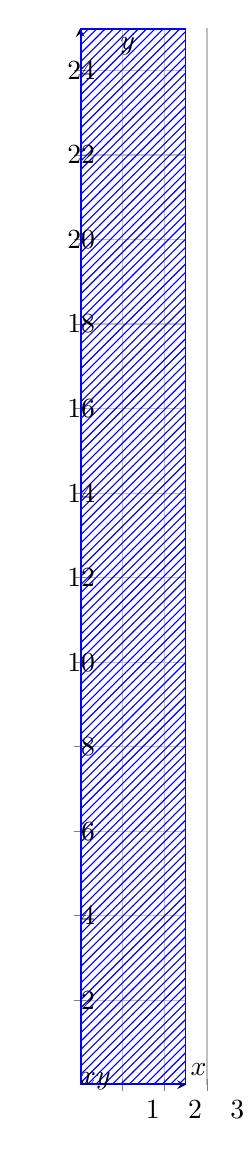
\begin{tikzpicture}

\begin{axis}[
            width=15cm,
            height=15cm,
            axis equal image,
            axis lines=middle,
            grid=major,
            enlargelimits=false,
            clip=true,
            xlabel=$x$,
            ylabel=$y$,
            domain=0.0:2.5,
            ymin=0.0,ymax=25.0,
            view={0}{90},
            samples=200
            ]
        

            width=15cm,
            height=15cm,
            axis equal image,
            axis lines=middle,
            grid=major,
            enlargelimits=false,
            clip=true,
            xlabel=$x$,
            ylabel=$y$,
            domain=0.0:2.5,
            ymin=0.0,ymax=25.0,
            view={0}{90},
            samples=200
            ]
        

            \addplot[
                name path=lowerBound0,
                domain=0.0:2.5,
                samples=200,
                draw=none 
            ] {0};

            \addplot[
                name path=upperBound0,
                domain=0.0:2.5,
                samples=200,
                draw=none 
            ] {25};

            \addplot[ 
                pattern=north east lines,
                pattern color=blue,
                draw= blue,
                line width=1pt
            ] fill between[
                of=lowerBound0 and upperBound0,
                soft clip={domain=0.0:2.5}
            ];

        
\end{axis}
\end{tikzpicture}
\end{center}

\end{document}
